\chapter{Weather Research and Forecast (WRF)}
\section{Aspectos Generales}
El modelo ARW-WRF (Advanced Research WRF) es un modelo atmosférico (es decir, simula el comportamiento de la atmósfera) no hidrostático que resuelve el sistema de ecuaciones para flujo compresible en su forma conservativa y utilizando una coordenada vertical de masa (o de presión hidrostática). Su coordenada vertical está definida como:
\begin{equation}
\eta = \frac{p_{dh}-p_{dht}}{\mu_d}
\end{equation}
Donde $p_{dh}$ corresponde a la componente hidrostática de la presión del aire seco, y:
\begin{equation}
\mu_d = p_{dhs} - p_{dht}
\end{equation}
es la masa de aire seco para una columna. En estas ecuaciones los subíndices $t$ y $s$ corresponden a los límites superior (top) e inferior (surface) del dominio. 

\begin{figure}[h!]
	\centering
	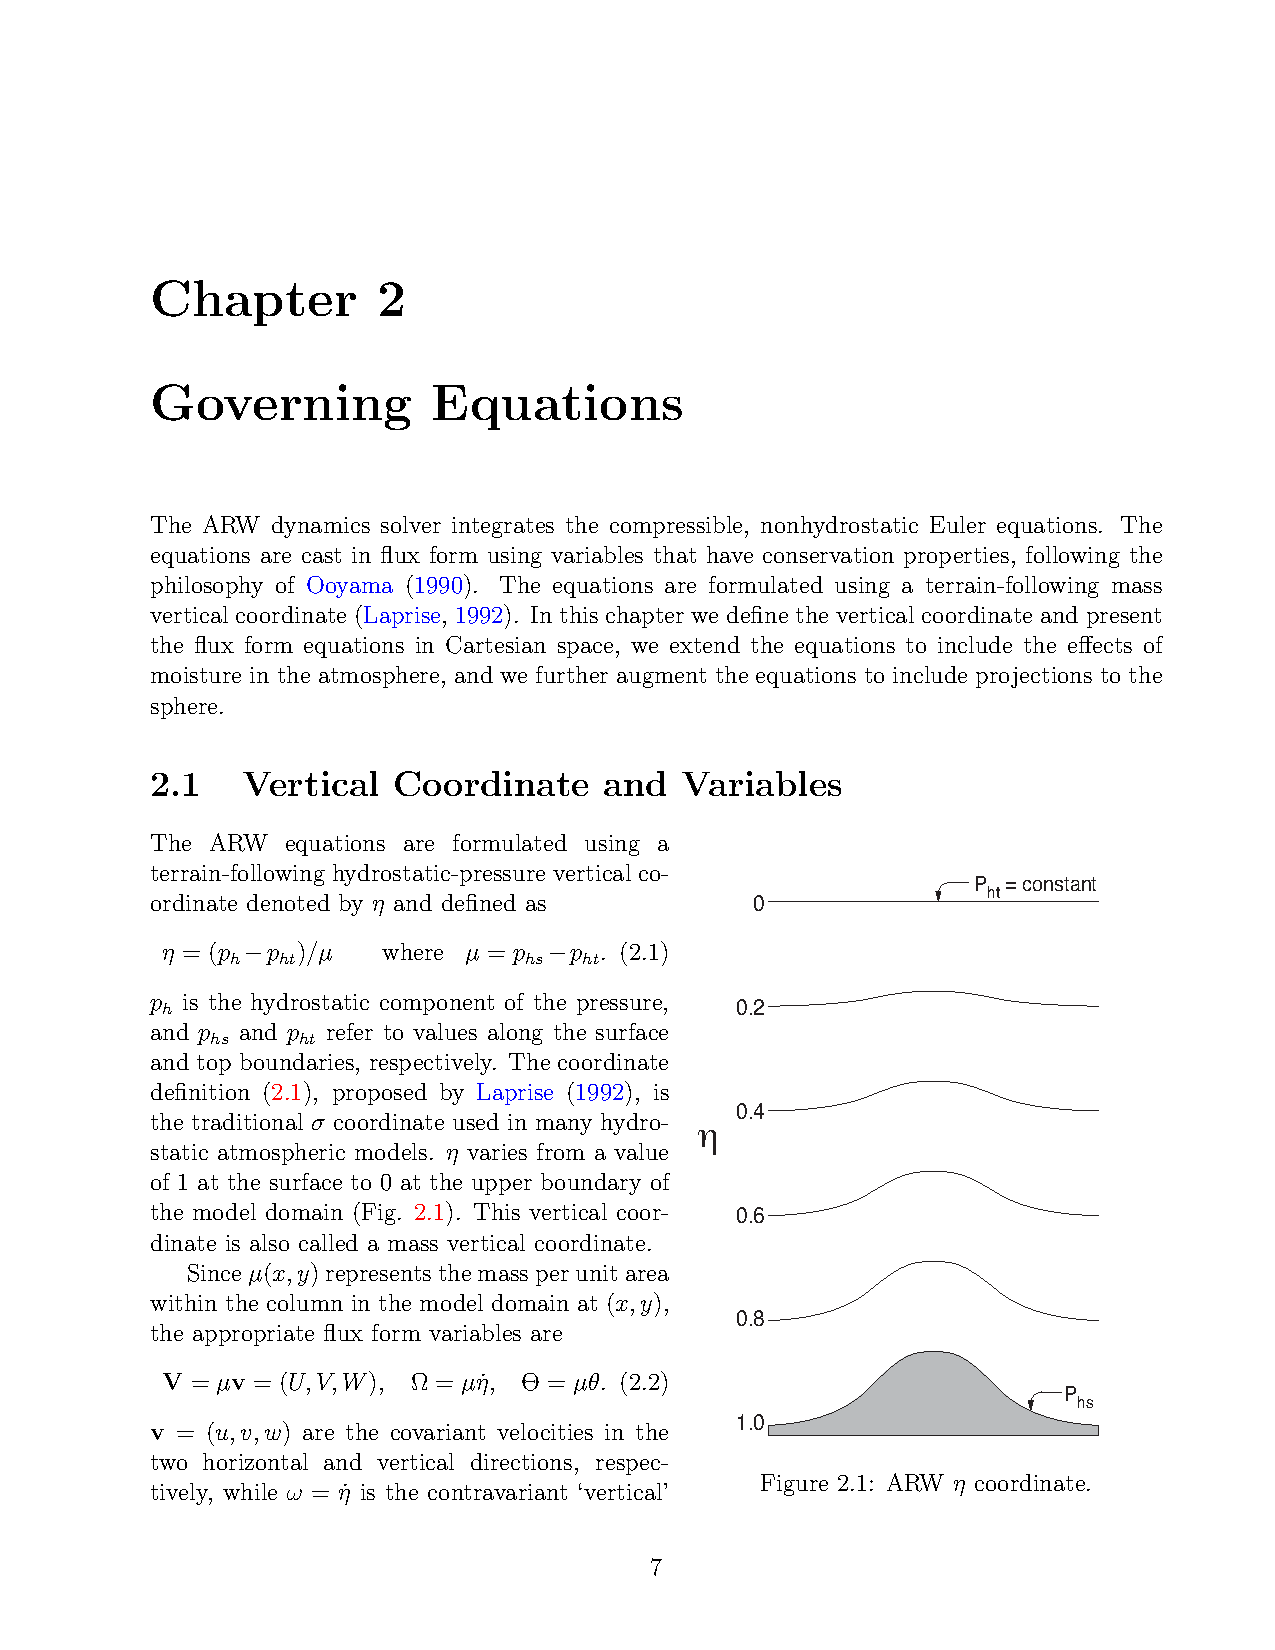
\includegraphics[width=0.55\linewidth,trim={11.5cm 3.3cm 1cm 14cm},clip]{Imagenes/eta}
	\caption{Estructura de la coordenada vertical.}
	\label{fig:eta}
\end{figure}

Las variables principales que resuelve el modelo son las velocidades covariantes $(u,v,w)$, masa de aire seco, el geopotencial, temperatura potencial ($\theta$) y energía cinética turbulenta (TKE) de submalla (SGS). La ecuación de momentum, temperatura potencial, SGS TKE y otros escalares relevantes tienen una forma acoplada con la masa de aire seco, de la forma:
\begin{equation}\label{eq:ec_conervacion}
\partial_t (\mu_d\theta) + \partial_x(\mu_d u \theta)+\partial_y(\mu_d v \theta)+\partial_\eta (\mu_d \omega \theta) = F
\end{equation}
Donde $F$ es la suma de la mezcla turbulenta junto con otras fuerzas y
\begin{equation}
\omega = d_t\eta
\end{equation}

es la velocidad en la coordenada vertical. Notar que la ecuación \ref{eq:ec_conervacion} corresponde a una ecuación de conservación de un escalar pasivo. $\theta$ es la temperatura potencial.

La discretización en el tiempo se realiza a través de un esquema de integración temporal múltiple. Este esquema separa los modos de alta frecuencia (i.e. ondas acústicas y de gravedad) de los modos de baja frecuencia (modo físico). ARW utiliza un esquema RK3 y durante cada paso en el RK, el modo de alta frecuencia que se propaga horizontalmente es integrado a través de un esquema \emph{forward-backward} utilizando un paso de tiempo acústico, que es típicamente un orden de magnitud mas pequeño que el paso físico, mientras que un esquema implícito es utilizado para el modo de alta frecuencia que se propaga de manera vertical.
\subsection{Ecuaciones Resueltas}
ecuaciones de euler, derivacion de las ecuaciones completas, etc.
\subsection{Discretización Espacial}
malla vertical, malla horizontal, arakawa c-grid, metodos anidados
\subsection{Discretización Temporal}
pasos de tiempo físico y acustico, pasos del rk3
\subsection{Aspectos Numéricos}
\subsubsection{Filtros}
filtro acustico, filtro polar, otros filtros
\subsubsection{Advección}
discretizacion numerica de la adveccion, limitadores, etc.
\subsubsection{Difusión}
La difusión y los flujos turbulentos calculados según el espacio físico $(x,y,z)$ se calculan haciendo uso de la métrica del espacio:
\begin{eqnarray}
z_x=g^{-1}\delta_x\phi \\
z_y=g^{-1}\delta_y\phi
\end{eqnarray}

El término difusivo se agrega al lado derecho de las ecuaciones de Euler, junto al resto de las fuerzas externas. Estas se ven:
\begin{eqnarray}
\partial_t U = \ldots - m_x[\partial_x\tau_{11}+\partial_y\tau_{12}-\partial_z(z_x\tau_{11}+z_y\tau_{12})]-\partial_z\tau_{13} \\
\partial_t V = \ldots - m_y[\partial_x\tau_{12}+\partial_y\tau_{22}-\partial_z(z_x\tau_{12}+z_y\tau_{22})]-\partial_z\tau_{23} \\
\partial_t W = \ldots - m_y[\partial_x\tau_{13}+\partial_y\tau_{23}-\partial_z(z_x\tau_{13}+z_y\tau_{23})]-\partial_z\tau_{33}
\end{eqnarray}

Y el tensor de esfuerzos viscosos es:
\begin{equation}
\tau_{ij} = -\mu_d K_{h,v}S_{ij}
\end{equation}
donde $K_{h,v}$ es la viscosidad turbulenta en dirección horizontal o vertical según la ecuación y $S_{ij}$ es el tensor tasa de deformación.

Para las malla no LES:
\begin{equation}
K_h = C_s^2 l^2[0.25(D_{11}-D_{22})^2+D_{12}]^{0.5}
\end{equation}
Con $C_s=0.25$ y $l=\sqrt{\Delta x\Delta y}$. $K_v$ queda definido según el esquema de parametrización utilizado para la capa límite planetaria.

Para las mallas con LES
la viscosidad turbulenta se calcula en función de la energía cinética turbulenta $e$ de la forma:
\begin{equation}
K_{h,v}=C_k l_{h,v}\sqrt{e}
\end{equation}
donde $C_k$ es una constante (normalmente $0.15<C_k<0.25$) y $l$ es un largo característico que se calcula en función de la isotropía de la malla, la resolución, $e$ y la estratificación de la forma:
\begin{align}
	l_v &= \min[\Delta z, 0.76\sqrt{e}/N]\quad&;&\quad N^2>0\\
	l_h &= \Delta z\quad&;&\quad N^2\leq 0
\end{align}
$N$ es la frecuencia de Brunt-Väisälä. $N=\sqrt{g/\theta d_z\theta}$

La clausura del modelo de turbulencia se hace considerando la ecuación de transporte para $e$ como:
\begin{equation}
\partial_t(\mu_d e) + (\partial_i V_i e)_\eta = \mu_d(\text{ producción + flotación + disipación})
\end{equation}
Con:
\begin{align}
	\text{Producción}&= K_h (D_{11}^2 + D_{22}^2 + D_{12}^2) + K_v (D_{33}^2 + D_{13}^2 + D_{23}^2)\\
	\text{Flotación}&=-K_v N^2\\
	\text{Disipación}&=-\frac{C e^{3/2}}{l}
\end{align}
\begin{align}
	C &= 1.9C_k + \frac{(0.93 - 1.9 C_k)l}{(\Delta x \Delta y \Delta z)^{1/3}}\\
	l &= \min[(\Delta x \Delta y \Delta z)^{1/3}, 0.76\sqrt{e}/N]
\end{align}
\subsubsection{Microfísicas}
detallar cada microfísica y su incorporacion a las ecuaciones